\section{Auswertung}
\label{sec:Auswertung}
\subsection{Temperaturverläufe}
%Tabelle der gemessenen Temperaturen 
\begin{table}
	\centering
	\sisetup{table-format=2.3}
	\begin{tabular}{S[table-format=1.2] S[table-format=1.3] S[table-format=1.3] }
	\toprule
	\multicolumn{1}{c}{Zeit} & {Temperaturen} \\
	{$t/\:\si{\minute}$} & {$T_1/\:\si{\kelvin}$} & {${T_2}/\:\si{\kelvin}$} \\
	\midrule

 0 & 294.45 & 294.45 \\
 1 & 295.35 & 294.45 \\
 2 & 296.15 & 294.35 \\
 3 & 297.45 & 293.45 \\
 4 & 299.05 & 292.05 \\
 5 & 300.85 & 290.25 \\
 6 & 302.95 & 288.25 \\
 7 & 304.85 & 286.45 \\
 8 & 306.85 & 284.65 \\
 9 & 308.65 & 282.85 \\
10 & 310.55 & 281.15 \\
11 & 312.25 & 279.45 \\
12 & 314.05 & 277.75 \\
13 & 315.65 & 276.35 \\
14 & 317.35 & 274.95 \\
15 & 318.85 & 273.95 \\
16 & 320.35 & 273.35 \\
17 & 321.75 & 272.85 \\
18 & 322.95 & 272.45 \\
19 & 324.15 & 272.05 \\
	\bottomrule
	\end{tabular}
	\caption{Zeitabhängige Messung der Temperaturen $T_1$ und $T_2$.}
	\label{tab:Temperaturverlauf}
\end{table}

Die gemessenen Temperaturen $T_1$ (rot) und $T_2$ (blau) der Reservoire werden gegen die Zeit $t$ aufgetragen, um einen ersten Eindruck des Temperaturverlaufes innerhalb der Reservoire zu gewinnen. Dabei ist Reservoir $R_1$ das Behältnis, welches die Wärmemenge $\mathup{d}Q_1$ aufnimmt und sich dabei erhitzt; $R_2$ (blau) bezeichnet das kälter werdende Reservoir.  Werden die Verläufe in einem gemeinsamen Diagramm dargestellt, so lassen sich diese untereinander vergleichen. 
\newpage
\begin{figure}
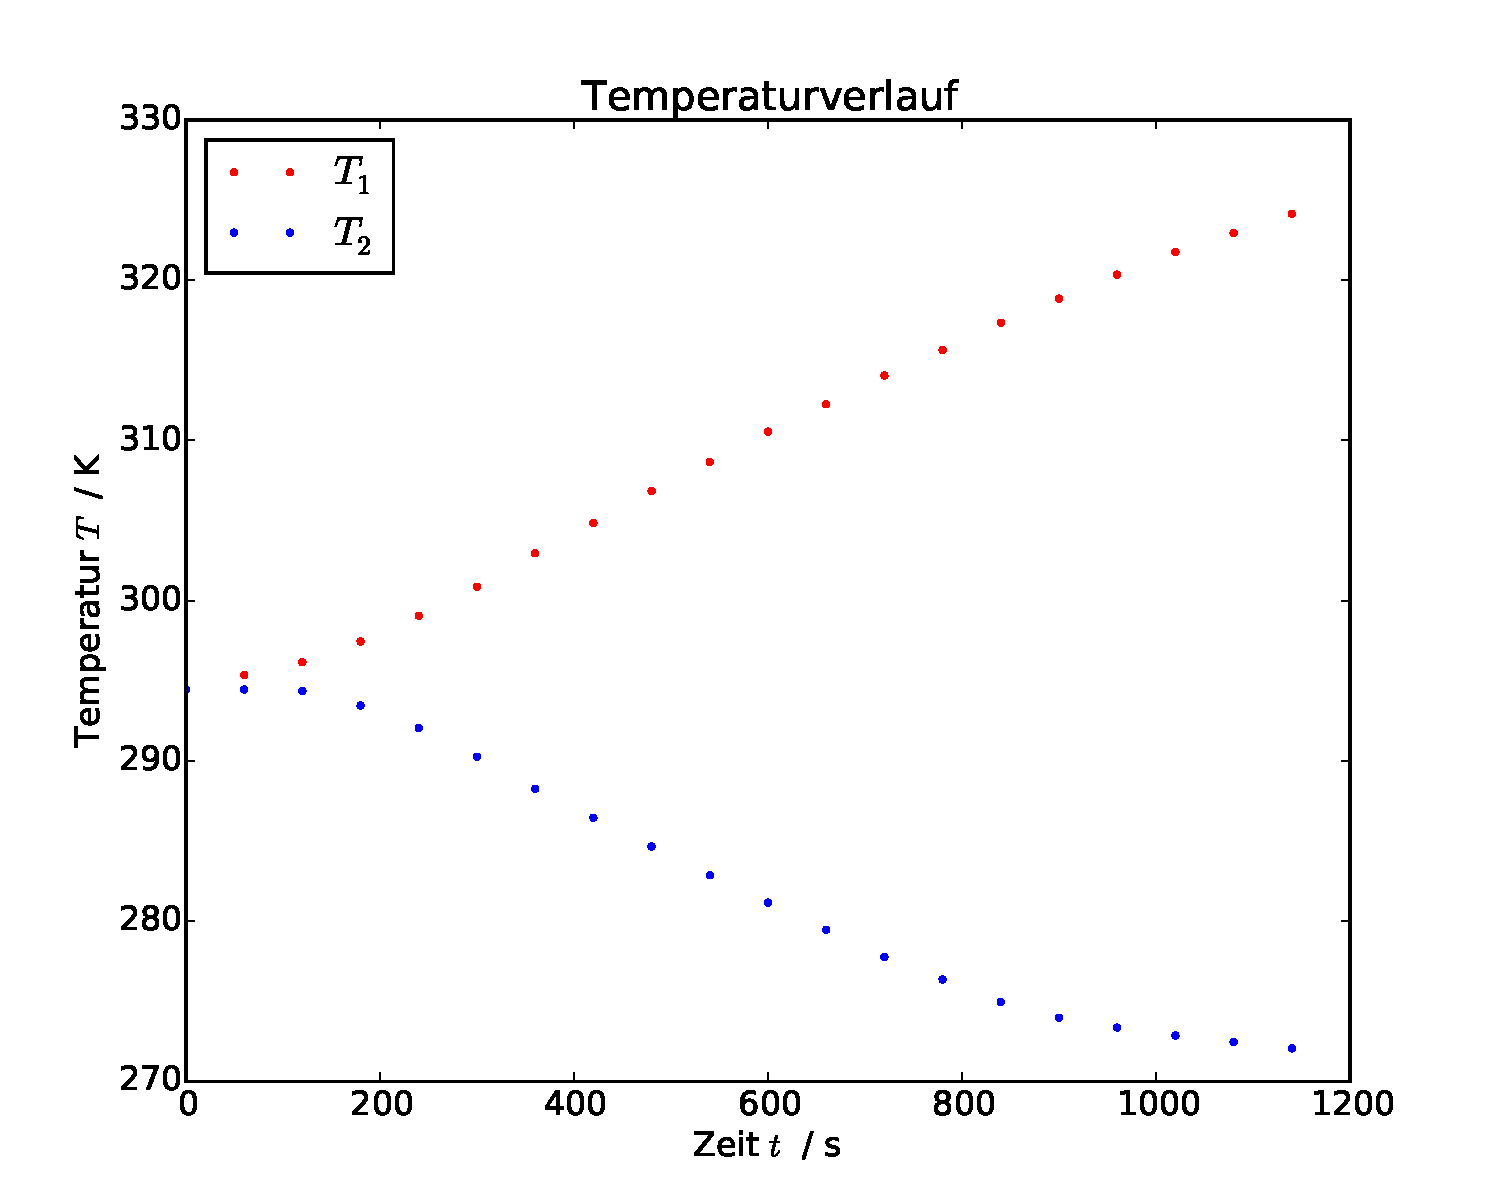
\includegraphics[width=\textwidth]{Bilder/Temperaturverlauf.pdf}
	\caption{Entwicklung der Wassertemperatur in den Reservoiren $\mathup{R_1}$ und $\mathup{R_2}$.}
	\label{fig:temperaturverlauf}
\end{figure}


Entgegen der Anweisung der Anleitung werden die Verläufe nicht durch eine nicht - lineare Ausgleichsrechnung mit
\begin{equation}
	T_i(t)=A_i t² + B_i t + C_i , i=1,2
	\label{eq:t-verlauf_Grad2}
\end{equation}
 -- einem Polynom zweiten Grades mit den Konstanten $A$, $B$ und $C$ -- genähert. Trotz zweiter Ordnung erscheint der Fit annähernd linear. Da schon anhand der Messwerte zu erkennen ist, dass diese einen Wendepunkt aufweisen wird ein Polynom dritten Grades benutzt; die Messwerte liegen deutlich weniger von der Näherung entfernt ( vgl. Abbildung 2, 3).

\begin{equation}
	T_i(t)=A_i t³ + B_i t² + C_i t + D_i , i=1,2
	\label{eq:t-verlauf_Grad3}
\end{equation}
\newpage
\begin{figure}
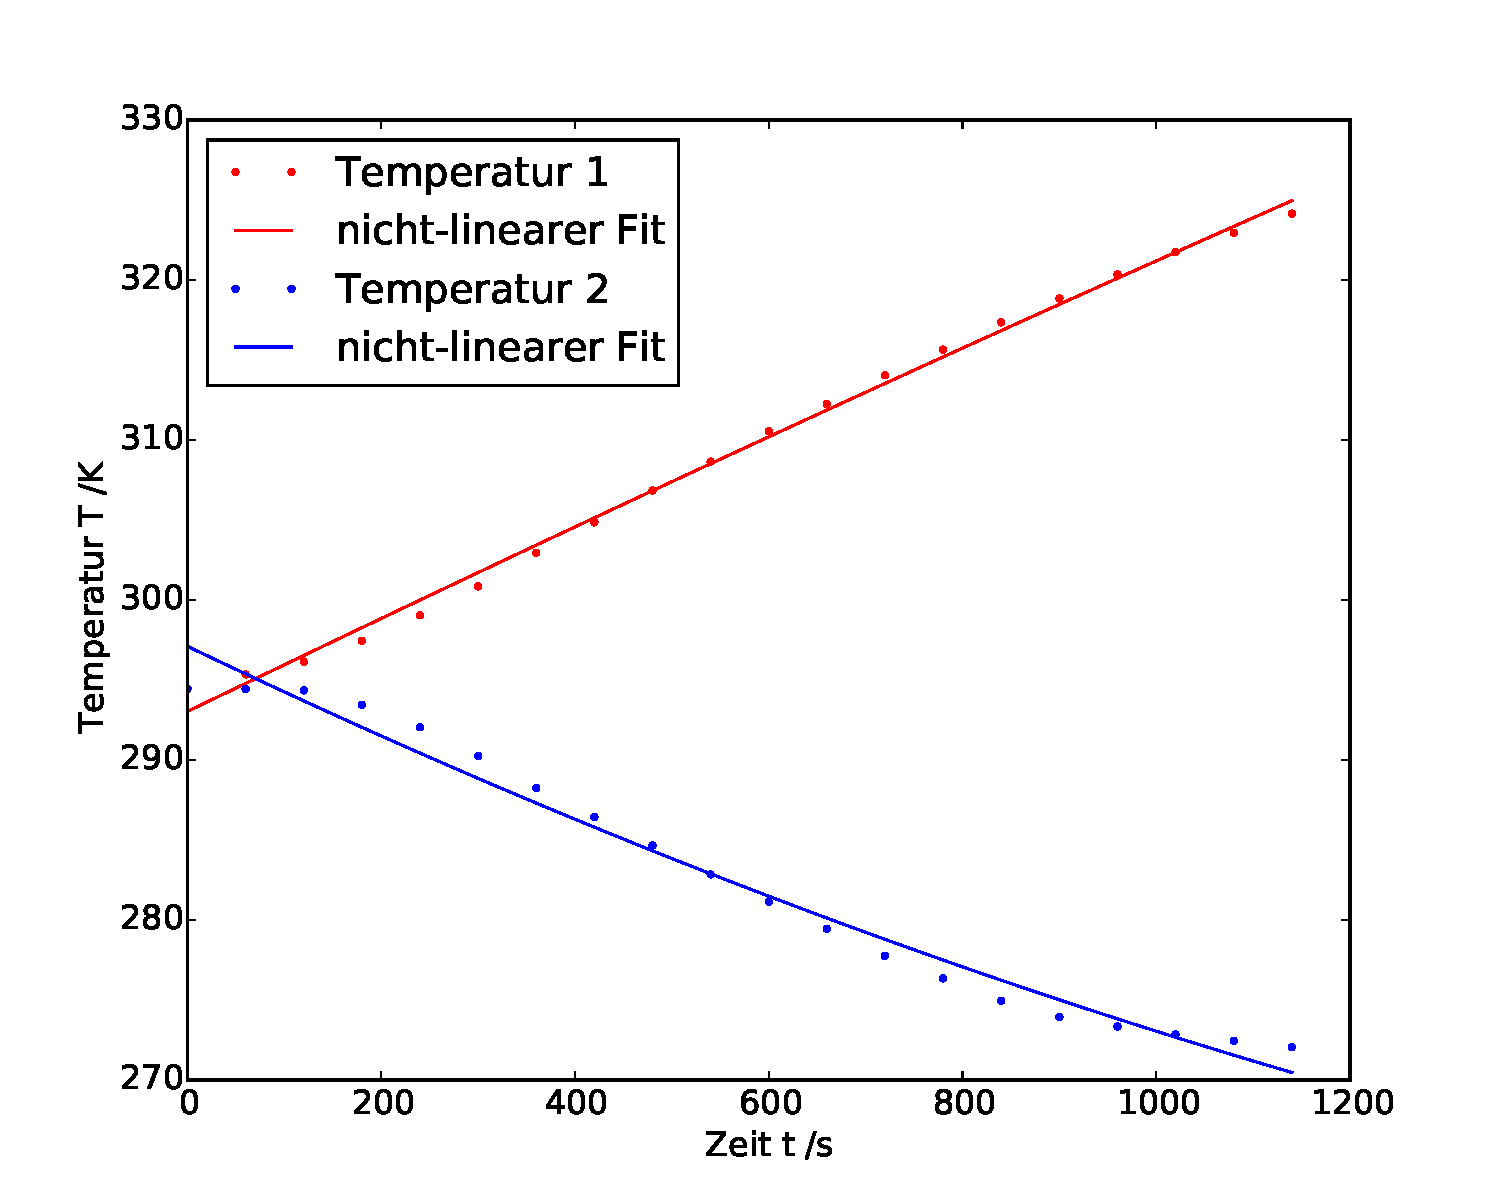
\includegraphics[width=\textwidth]{Bilder/Temperaturfit_Grad2.pdf}
	\caption{Annäherung der Kurven durch ein Polynom zweiter Ordnung.}
\end{figure}

\begin{figure}
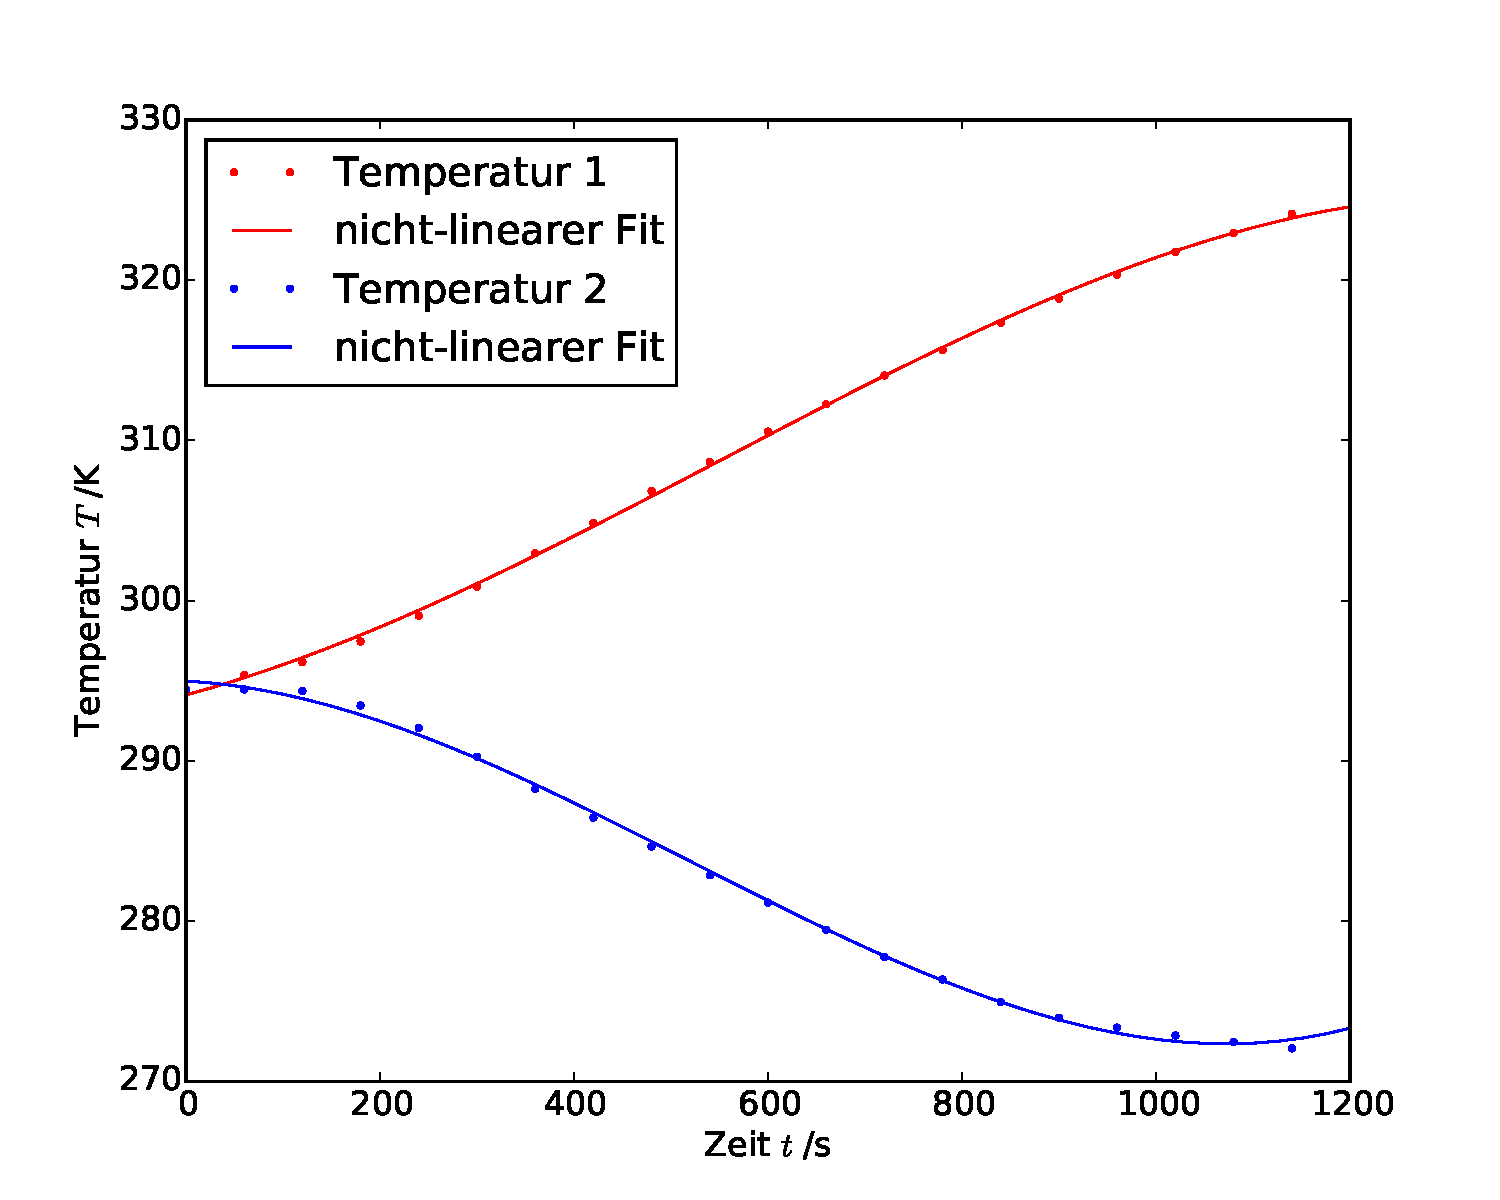
\includegraphics[width=\textwidth]{Bilder/Temperaturfit.pdf}
	\caption{Annäherung der Kurven durch ein Polynom dritter Ordnung.}
\end{figure}
\newpage
Es ergeben sich für $T_1(t)$ und $T_2(t)$ die Koeffizienten 
\begin{equation}
\begin{split}
A_1&=(-1.72\pm0.18)10⁻⁸\si{\kelvin\per{\second}³}\\
B_1&=(2.82\pm0.31)10⁻⁵\si{\kelvin\per{\second}²}\\
C_1&=(0.0162\pm0.0015)\si{\kelvin\per{\second}}\\
D_1&=(294.11\pm0.19)\si{\kelvin}
\end{split}
\end{equation}
und
\begin{equation}
\begin{split}
A_2&=(3.39\pm0.25)10⁻⁸\si{\kelvin\per{\second}³}\\
B_2&=(-5.30\pm0.43)10⁻⁵\si{\kelvin\per{\second}²}\\
C_2&=(-0.0033\pm0.0021)\si{\kelvin\per{\second}}\\
D_2&=(294.98\pm0.27)\si{\kelvin}.
\end{split}
\end{equation}

Um den Differentialqutionenten $\frac{\mathup{d}T_i}{\mathup{d}t}$ mit $i=1,2$ für verschiedene Zeiten $t_k$ mit $k=1,...,4$ bestimmen zu können, wird die Funktion $T_i(t)$ nach der Zeit $t$ abgeleitet und die Fehler der Gradienten mittels Gaußscher Fehlerfortpflanzung berechnet:

\begin{equation}
\frac{\mathup{d}T_i}{\mathup{d}t}= 3A_it²+2B_it+C_i.
\label{ableitung}
\end{equation}

\begin{table}
	\centering
	
	\begin{tabular}{S S S}
	\toprule
	\multicolumn{1}{c}{Zeit} & \multicolumn{2}{c}{Differentialquotienten} \\
	{$t/\:\si{\second}$} & {$\frac{\mathup{d}T_1}{\mathup{d}t}/\:\si{\kelvin{\per\second}}$} & {$\frac{\mathup{d}T_2}{\mathup{d}t}/\:\si{\kelvin{\per\second}}$}\\
	\midrule
 120 & 0.022 $\pm$ 0.002   & -0.015 $\pm$0.002  \\
 480 & 0.032 $\pm$ 0.004   & -0.031 $\pm$ 0.005  \\
 840 & 0.027 $\pm$ 0.007   & -0.021 $\pm$ 0.009  \\
1080 & 0.017 $\pm$ 0.009   &  0.001 $\pm$ 0.013  \\
	\bottomrule
	\end{tabular}
	\caption{Die Differentialqutienten von $T_1$ und $T_2$ zu vier verschiedenen Zeiten $t_k$, berechnet nach Gleichung \eqref{ableitung}.}
	\label{tab:differentialquotienten}
\end{table}

%%%%%%%%%%%%%%%%%%%%%%%%%%%%%%%%%%%%%%%%%%%%%%%%%FEHLERRECHNUNG NACH GAUSS:FORMEL FEHLT NOCH!!!!!!!!!!!!!!!!!


\subsection{Bestimmung der Güteziffer}
Die reale Güteziffer $\nu$ wird mit Hilfe der Messreihe $T_1$  über den Differenzenquotienten $\frac{\Delta{T_1}}{\Delta{t}}$, die Wärmemenge $\Delta{Q_1}$, welche im Zeitintervall $\Delta{t}$ dem ersten Reservoir zugeführt wird, multipliziert mit dem Kehrwert des Mittelwertes der Kompressorleistung $N_\mathup{el.}$, berechnet mit
%das vielleicht noch in die Theorie einbringen??
\begin{equation}
\nu_\mathup{real}=\frac{\Delta{Q_1}}{{\Delta{t}}N_\mathup{el.}}=(m_1c_\mathup{w}+m_\mathup{k}c_\mathup{k})\frac{\Delta{T_1}}{{\Delta{t}}N_\mathup{el.}}.
\label{waermemenge/zeitintervall}
\end{equation}

Die Konstanten $m_1c_\mathup{w}=4.183 10⁻³\:\si{\joule\per{\kelvin\kilo\gram}}$ und $m_\mathup{k}c_\mathup{k}=660\:\si{\joule\per\kelvin}$ sind die Wärmekapazitäten des verwendeten Wassers und der kupfernen Heizspirale. Die Gesamtkapazität bei $3\si\liter$ Wasservolumen ist $m_1c_\mathup{w}+m_\mathup{k}c_\mathup{k}=13209\:\si{\joule\per\kelvin}$.

Die Fehlerangaben der werden berechnet mit
\begin{equation}
\Delta{\nu_\mathup{real}}=\sqrt{\biggl(\frac{(m_1c_\mathup{w}+m_\mathup{k}c_\mathup{k})\frac{\mathup{d}T_1}{\mathup{d}{t}}}{N_t}\biggr)^2+\biggl(\frac{(m_1c_\mathup{w}+m_\mathup{k}c_\mathup{k})\Delta{T_1}}{(N_t)^2 \Delta{t}}\Delta{N_t}\biggr)^2}
\end{equation}

Dabei ist $\Delta{N_t}$ der mittelre Fehler von $N_t$, dem Mittel der Kompressorleistung der Zeiten $t$ (gvl. \ref{tab:differentialquotienten}. Beides wird berechnet durch

\begin{equation}
	N_t=\frac{1}{n}\sum_{k=0}^n{(N_k-N)²}
\end{equation}
\begin{equation}
	\Delta{N_t}=\sqrt{\frac{\frac{1}{n-1}\sum_{k=0}^n(N_k)}{n}}.
\end{equation}

Die ideale Güteziffer $\nu_\mathup{ideal}$ wird nach Gleichung \eqref{eq:nu_ideal} zum Vergleich ebenfalls berechnet.


%\begin{table}
%	\centering
	
	%\begin{tabular}{S S S}
	%\toprule
	%\multicolumn{1}{c}{Zeit} & \multicolumn{2}{c}{Güteziffern} \\
	%{$t/\:\si{\second}$} & {$\nu_\mathup{ideal}$} & {$\nu_\mathup{real}$}\\
	%\midrule
 %120 & 0.022 $\pm$ 0.002   & -0.015 $\pm$0.002  \\
 %480 & 0.032 $\pm$ 0.004   & -0.031 $\pm$ 0.005  \\
 %840 & 0.027 $\pm$ 0.007   & -0.021 $\pm$ 0.009  \\
%1080 & 0.017 $\pm$ 0.009   &  0.001 $\pm$ 0.013  \\
%	\bottomrule
%	\end{tabular}
%	\caption{Die Differentialqutienten von $T_1$ und $T_2$ zu vier verschiedenen Zeiten $t_k$, berechnet nach Gleichung \eqref{ableitung}.}
%	\label{tab:differentialquotienten}
%\end{table}


